\section{Existence of Ramsey Numbers}
This section is based upon \cite{rt}[Section 1.1].
\begin{definition}
	Let $\ell_1, \ell_2, \ldots, \ell_r, n \in \mathbb{N}^{+}$ we will write $n \to (\ell_1, \ell_2, \ldots, \ell_{r})$ if for every $r$-edge coloring $\chi: E(K_{n}) \to \left\{c_1, c_2, \ldots, c_{r}\right\}$ on $K_n$, there exists an $i \in \left\{1, 2, \ldots, r\right\}$ such that $\chi$ admits a $c_{i}$-monochromatic clique of order $\ell_{i}$.
\end{definition}
\begin{remark}
	Clearly $\ell_i \geq \ell_i'$ and $n \to (\ell_1, \ell_2, \ldots, \ell_{r})$ implies that $n \to (\ell_1', \ell_2', \ldots, \ell_{r}')$, since given an $r$-edge coloring $\chi: E(K_{n}) \to \left\{c_1, c_2, \ldots, c_{r}\right\}$ on $K_{n}$ there exists an $i \in [r]$ such that $K_n$ has a $c_{r}$-monochromatic clique of order $\ell_{i} \geq \ell_{i}'$.
\end{remark}

\begin{theorem}[Ramsey's Theorem]\label{thm:ramsey_two_colors}
	Let $\ell_1, \ell_2 \geq 2$, then there exists a $n \in \mathbb{N}^{+}$ such that $n \to (\ell_1, \ell_2)$.
\end{theorem}
\begin{proof}
	Clearly $\ell_1 \to (\ell_1, 2)$ and $\ell_2 \to (2, \ell_2)$ (after all either $K_{\ell_{i}}$ is monochromatic or there exist a monochromatic clique of order $2$). We will proceed using induction on $\ell_1 + \ell_{2}$, hence we may assume that $\ell_1 + \ell_2 \geq 6$, with $\ell_1, \ell_2 \geq 3$.
	Additionally by our induction hypothesis we may assume the existence of non-zero $n_1, n_2 \in \mathbb{N}$ such that $n_1 \to (\ell_1, \ell_2 - 1)$ and $n_2 \to (\ell_1 - 1, \ell_2)$. Next let $n := n_1 + n_2$ we will show that $n \to (\ell_1, \ell_2)$. Fix an arbitrary $2$-edge coloring $\chi: E(K_{n}) \to \left\{red, blue\right\}$ on $K_n$ and let $v$ be a vertex in $K_n$, then $v$ is adjacent to $n - 1$ other vertices in $K_{n}$, hence:
	\begin{equation*}
		n_1 + n_2 - 1 = n - 1 = \abs{\mathcal{N}_{\chi}(v; red)} + \abs{\mathcal{N}_{\chi}(v; blue)}
	\end{equation*}
	meaning either $\abs{N_{\chi}(v; red)} \geq n_2$ or $\abs{N_{\chi}(v; blue)} \geq n_1$, by the Generalized Pigeonhole Principle (Theorem \ref{thm:gpp}). Without loss of generality assume that the second inequality holds, namely $\abs{N_{\chi}(v; blue)} \geq n_1$. By our inductive hypothesis, the complete graph:
	\begin{equation*}
		G = \left(N_{\chi}(v; blue), E(K_{n}) \cap (N_{\chi}(v; blue) \times N_{\chi}(v; blue))\right)
	\end{equation*}
	contains either a $red$-monochromatic clique of order $\ell_{1}$ (in which case we are done) or a $blue$-monochromatic clique of order $\ell_{2} - 1$, in which case we note that $v$ is connected to the vertices in $N_{\chi}(v; 2)$ via edges which $\chi$ colors $blue$, and hence $K_n |_{\mathcal{N}_{\chi}(v, blue) \cup \left\{v\right\}}$ is a $blue$-monochromatic clique of order $\ell_{2}$.
\end{proof}

\begin{corollary}\label{cor:ramsey_for_arbitarily_many_colors}
	Let $\ell_1, \ell_2, \ldots, \ell_r \geq 2$, then there exists a $n \in \mathbb{N}^{+}$ such that $n \to (\ell_1, \ell_2, \ldots, \ell_{r})$.
\end{corollary}

\begin{proof}
	We proceed using induction on $r$, the base case $r = 2$ is proven in Theorem \ref{thm:ramsey_two_colors}.
	Next assume that the theorem holds for $r - 1$. From Theorem \ref{thm:ramsey_two_colors}, it follows that there exists a $\ell \in \mathbb{N}^{+}$ such that $\ell \to (\ell_{r - 1}, \ell_{r})$.
	By our induction hypothesis we may find a $n \in \mathbb{N}^{+}$ for which it holds that:
	\begin{equation*}
		n \to (\ell_1, \ell_2, \ldots, \ell_{r - 2}, \ell)
	\end{equation*}
	Now given any $r$-edge coloring $\chi: E(K_n) \to \left\{c_1, c_2, \ldots, c_{r}\right\}$ on $K_n$ we may obtain a $r - 1$-edge coloring $\chi': E(K_{n}) \to \left\{c_1, c_2, \ldots, c_{r-1}\right\}$ on $K_n$ by defining:
	\begin{equation*}
		\chi'(e) = \begin{cases} \chi(e) & \text{ if } \chi(e) \neq c_{r} \\ c_{r - 1} & \text{ if } \chi(e) = c_{r} \end{cases}
	\end{equation*}
	Hence $\chi'$ must either admit a $c_{i}$-monochromatic clique of order $\ell_i$, for some $i \in \left\{1, 2, \ldots, r - 2\right\}$ (in which case we are done) or a $c_{r - 1}$-monochromatic clique of order $\ell$. If the second case holds let $C$ be this $c_{r-1}$-monochromatic clique of order $\ell$, then $\chi$ colors every edge in $C$ with either $c_{r - 1}$ or $c_{r}$. However $\ell$ was chosen so that $\ell \to (\ell_{r - 1}, \ell_r)$, hence $C$ must contain either a $c_{r - 1}$-monochromatic clique of order $\ell_{r - 1}$ or a $c_{r}$-monochromatic clique of order $\ell_{r}$.
\end{proof}

\begin{definition}
	Let $\ell_1, \ell_2, \ldots, \ell_r \in \mathbb{N}^{+}$ the \textit{Ramsey number} $R(\ell_1, \ell_2, \ldots, \ell_{r})$, is the minimal $n \in \mathbb{N}^{+}$ such that $n \to (\ell_1, \ell_2, \ldots, \ell_{r})$, additionally we let $R(\ell; r)$ denote $R(\ell_1, \ell_2, \ldots, \ell_{r})$, with $\ell_1 = \ell_2 = \cdots = \ell_r = \ell$. The Ramsey numbers of the form $R(\ell; 2)$ are called \textit{digaonal Ramsey numbers}.
\end{definition}
\begin{remark}
	The Ramsey number $R(\ell,k)$ can also be thought of as the minimum order an arbitrary graph $G = (V, E)$ must be, to guarantee the existence of a clique of order $\ell$ or a set of $k$ independent vertices, that is there exists a set $U$ of $k$ verticies such that no two verticies in $U$ are adjacent.
\end{remark}
Generally direct computation of Ramsey numbers are extremely difficult, however there is some exceptions, for instance we have $R(2, \ell) = R(\ell, 2) = \ell$, confer the basis step in the proof of Theorem \ref{thm:ramsey_two_colors}, below we present another example.

\begin{example}\label{exmp:R3_3}
	In this example we will show that $R(3, 3) = 6$, we start by showing that $R(3, 3) \leq 6$. Consider an arbitary $2$-edge coloring $\chi: E(K_{6}) \to \left\{red, blue\right\}$ on $K_6$ and let $v$ be a vertex in $K_6$, then $v$ has $5$ adjacent neighbours, by the generalized pigeonhole principle, Theorem \ref{thm:gpp}, there is a color $c$ (either $red$ or $blue$) such that $\abs{\mathcal{N}_{\chi}(v; c)} \geq 3$.

	Without loss of generality we may assume that $c = red$. Next take pairwise distinct $v_1, v_2, v_3 \in \mathcal{N}_{\chi}(v; red)$, then we must have $\chi(v_{i}, v_{j}) = blue$ for pairwise distinct $i, j \in [3]$, otherwise $K_{6} |_{\left\{v, v_i, v_j\right\}}$ would form a $red$-monochromatic clique of order $3$. However this in turn means that $\chi(v_i, v_j) = blue$ for all pairwise distinct $i, j \in [3]$, hence $K_6 |_{\left\{v_1, v_2, v_3\right\}}$ forms a $blue$-monochromatic clique of order $3$.

	On the other hand it is easy to construct a $2$-edge coloring on $K_5$ which admit no monochromatic subclique of order $3$, one example of such a $2$-edge coloring is illustrated in Figure \ref{fig:K5_counter_example}.
	\begin{figure}[H]
		\centering
		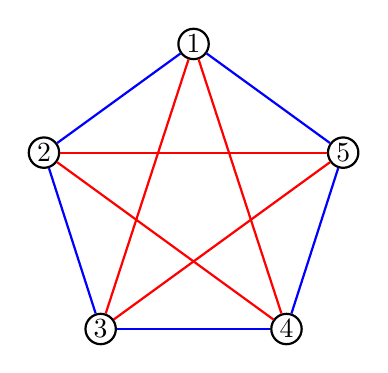
\begin{tikzpicture}
			\tikzset{punkt/.style={circle, thick, draw=black, minimum width=0.2cm,inner sep=1}}
			\node[punkt] at (0.0, 2.0) (a) {$1$};
			\node[punkt] at (-1.9, 0.62) (b) {$2$};
			\node[punkt] at (-1.18, -1.62) (c) {$3$};
			\node[punkt] at (1.18, -1.62) (d) {$4$};
			\node[punkt] at (1.9, 0.62) (e) {$5$};
			%\draw (0,0) circle [radius=2];

			% Blue edges
			\draw [thick, draw=blue] (a) -- (b);
			\draw [thick, draw=blue] (b) -- (c);
			\draw [thick, draw=blue] (c) -- (d);
			\draw [thick, draw=blue] (d) -- (e);
			\draw [thick, draw=blue] (e) -- (a);

			% Red edges
			\draw [thick, draw=red] (a) -- (c);
			\draw [thick, draw=red] (a) -- (d);
			\draw [thick, draw=red] (b) -- (d);
			\draw [thick, draw=red] (b) -- (e);
			\draw [thick, draw=red] (c) -- (e);
		\end{tikzpicture}
		\caption{A 2-edge coloring on $K_{5}$ that admits no monochromatic subclique of order $3$.}
		\label{fig:K5_counter_example}
	\end{figure}
	Finally since $R(3, 3) > 5$ and $R(3, 3) \leq 6$, we obtain that $R(3, 3) = 6$.
\end{example}
\newpage

We might also be interested in when an $r$-edge coloring of a complete graph admits some special monochromatic subgraphs, following this spirit we introduce the following definition:
\begin{definition}
	Let $G_1, G_2, \ldots, G_r$ be graphs, the \textit{generalized Ramsey number} $R(G_1, G_2, \ldots, G_{r})$ is the smallest integer $N$ such that for any $r$-edge coloring $\chi: E(K_N) \to \{c_1, c_2, \ldots, c_{r}\}$ there exists some index $i \in [1; r]$ such that there exists a $c_i$ monochromatic subgraph of $K_n$ which is isomorphic to $G_{i}$.
\end{definition}

It is worth noting that the generalized Ramsey number $R(G_1, G_2, \ldots, G_{r})$ is well defined. This can be seen as follows: let $\ell_j = \abs{V(G_{j})}$ consider the arbitrary $r$-coloring $\chi: E(K_n) \to \{c_1, c_2, \ldots, c_{r}\}$ of $K_n$ with $n = R(\ell_1, \ell_2, \ldots, \ell_{r})$. Then by the definition of $R(\ell_1, \ell_2, \ldots, \ell_{r})$ there exists an $i \in [1; r]$ such that $\chi$ admits a $c_i$-monochromatic clique of order $\ell_i$. The rest follows by the well ordering principle and the fact that $G_i$ is isomorphic to a subgraph of the previously mentioned $c_{i}$-monochromatic clique.
